\frame{
	\frametitle{Spatial Sort}
	%\todonaps{Spatial Sort}

	\begin{columns}
		\column{.6\textwidth}
			\begin{itemize}%\itemsep=20pt
				\item Points closer in space are more likely to follow a similar traversal;
				\item By sorting items, this can be exploited for temporal locality;
				\item Sorting using space-filling curves;
				\begin{itemize}
					\item Implemented using the CGAL library;
				\end{itemize}
			\end{itemize}
		
			\begin{figure}
				\centering
				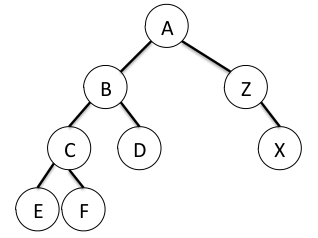
\includegraphics[width=0.5\columnwidth]{pointblocking_tree}
			\end{figure}

		\column{0.4\textwidth}

			\begin{figure}
				\centering
				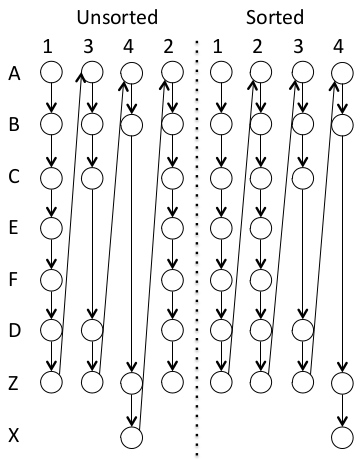
\includegraphics[width=0.9\columnwidth]{pointblocking_sort}
			\end{figure}
	\end{columns}

	\textbf{Fails when traversal depth is too large to fit in cache.}
}